\documentclass{beamer}
\usetheme{metropolis}
\usepackage{graphicx}
\usepackage{amsmath}
\title{A History of Science in Latin America (INTD290): Unit 1}
\author{Jordan Hanson}
\institute{Whittier College Department of Physics and Astronomy}

\begin{document}
\maketitle

\section{Review}

\begin{frame}{Review}
\begin{enumerate}
\item What is science?
\item Is science true?
\item Vocabulary in Nahuatl and Espa\~{n}ol
\item Geography
\item Scientific, Church, and Philosophical terminology
\end{enumerate}
\end{frame}

\section{Summary}

\begin{frame}{Summary}
\alert{Indigenous and Spanish Colonial Medicine}:
\begin{enumerate}
\item Indigenous medicine and science
\item Medieval medical theory
\begin{itemize}
\item The four humours
\item Hot/cold, wet/dry
\item Relation to elements, digestion
\end{itemize}
\item Comparisons of treatments: examples of indigenous science
\item Production of treatments
\begin{itemize}
\item Introduction from indigenous to colonial
\item Production and shipment to Europe
\end{itemize}
\end{enumerate}
\alert{Connections Activities}:
\begin{itemize}
\item The base-20 number system of the Maya
\item The Quipu of the Inca
\item Kepler's Laws
\end{itemize}
\end{frame}

\section{Indigenous Medicine and Science}

\begin{frame}{Indigenous Medicine and Science}
\small
\textbf{Huitzilin}: hummingbird.  A discussion of Linnaean classification.  This species is completely restricted to the New World, so it would have been totally unknown to colonials.
\begin{itemize}
\item quetzal huitzilin (a quetzal is not a hummingbird)
\item xi huitzilin ... turquiose hummingbird
\item chalchi huitzilin ... light greed hummingbird
\item yiauhtic huitzilin ... purple hummingbird
\item tlapal huitzilin ... mixed black hummingbird
\item aiopal huitzilin ... light purple hummingbird
\item tle huitzilin ... hot coal colored hummingbird
\item quapa huitzilin ... tawny yellow hummingbird
\end{itemize}
The Nahua believed that hummingbirds are symbols of the warrior and immortality (torpor).
\end{frame}

\begin{frame}{Indigenous Medicine and Science}
Here is what Father Diego Dur\'{a}n writes from conversations with Aztec people:
\begin{quote}
The sit on a branch next to the hollow, and stick their beak in it as far as they can and remain their for six months of the year - the entire winter - finding sustenance only on that tree, as if dead.  When spring comes and gets new growth and gets new leaves, the bird, helped by the vigor of the tree, resuscitates and goes forth and procreates. Because of this, the Indians say they die and are resurrected.  I have seen it with my own eyes in winter. 
\end{quote}
\url{https://youtu.be/8ObONmJ4VU8}
\end{frame}

\begin{frame}{Indigenous Medicine and Science}
\begin{figure}
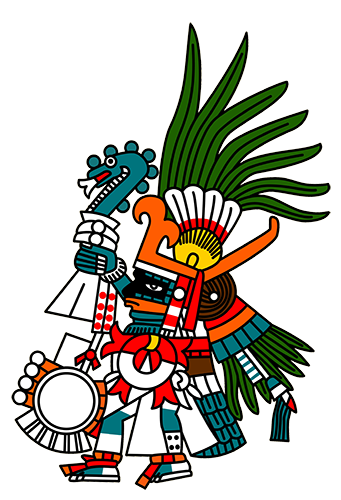
\includegraphics[width=3cm]{figures/aztec4.png} \hspace{1cm}
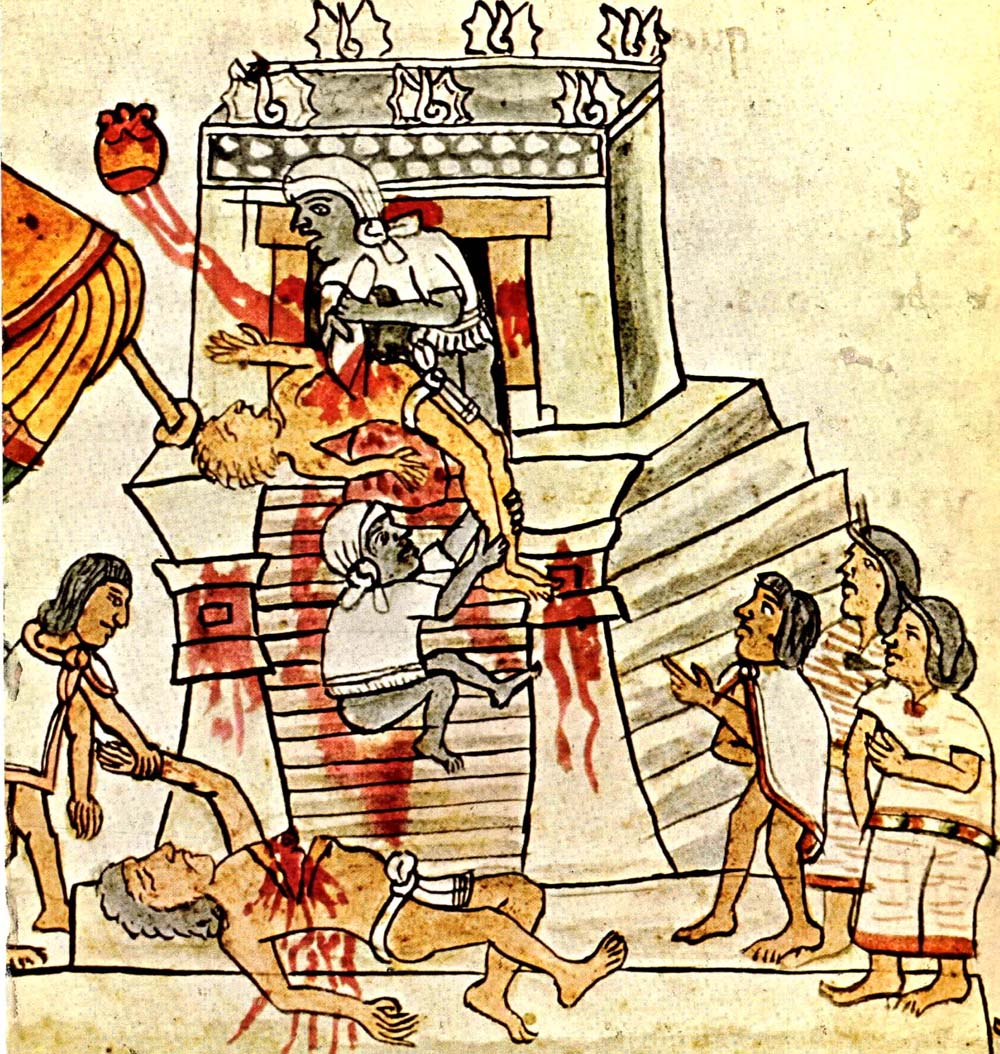
\includegraphics[width=3cm]{figures/sacrifice.jpg}
\caption{(Left) An icon of Huitzilopochtli, ``Southern hummingbird,'' or, ``Left-hand hummingbird.'' The Aztecs oriented the world so that South was to the left.  (Right) The Aztecs performed human heart sacrifices to Huitzilopochtli until the Spanish conquest.  (Mention the order of the words in huitzil + opochtli).}
\end{figure}
\end{frame}

\begin{frame}{Indigenous Medicine and Science}
\begin{figure}
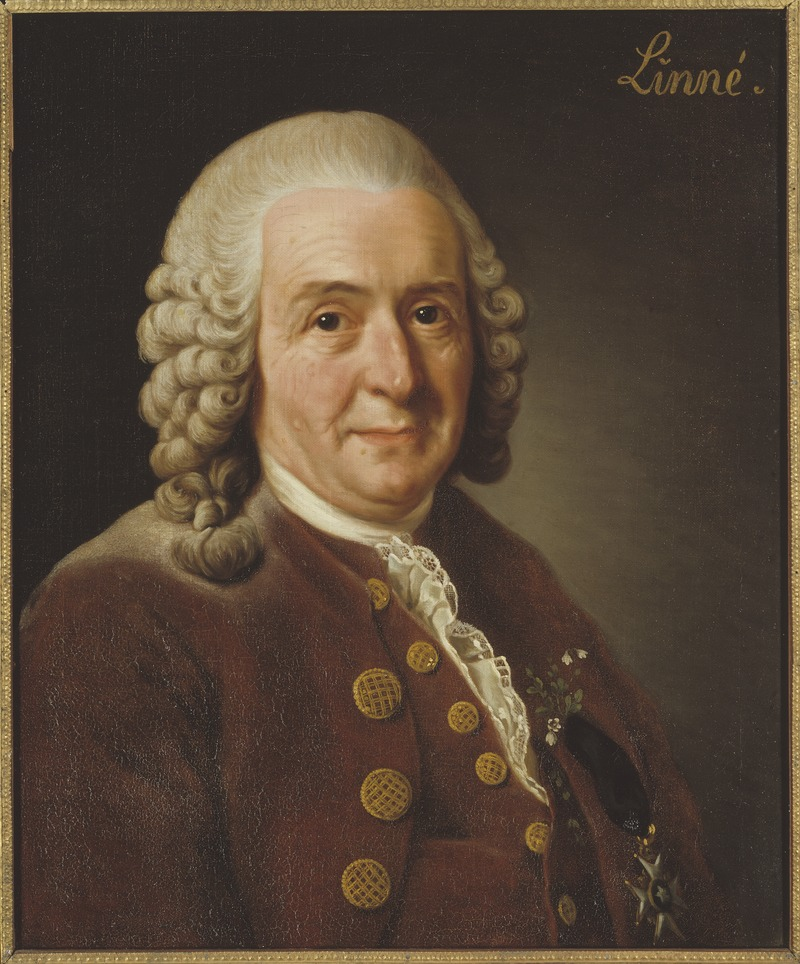
\includegraphics[width=2cm]{figures/linnaeus.jpg} \hspace{0.5cm}
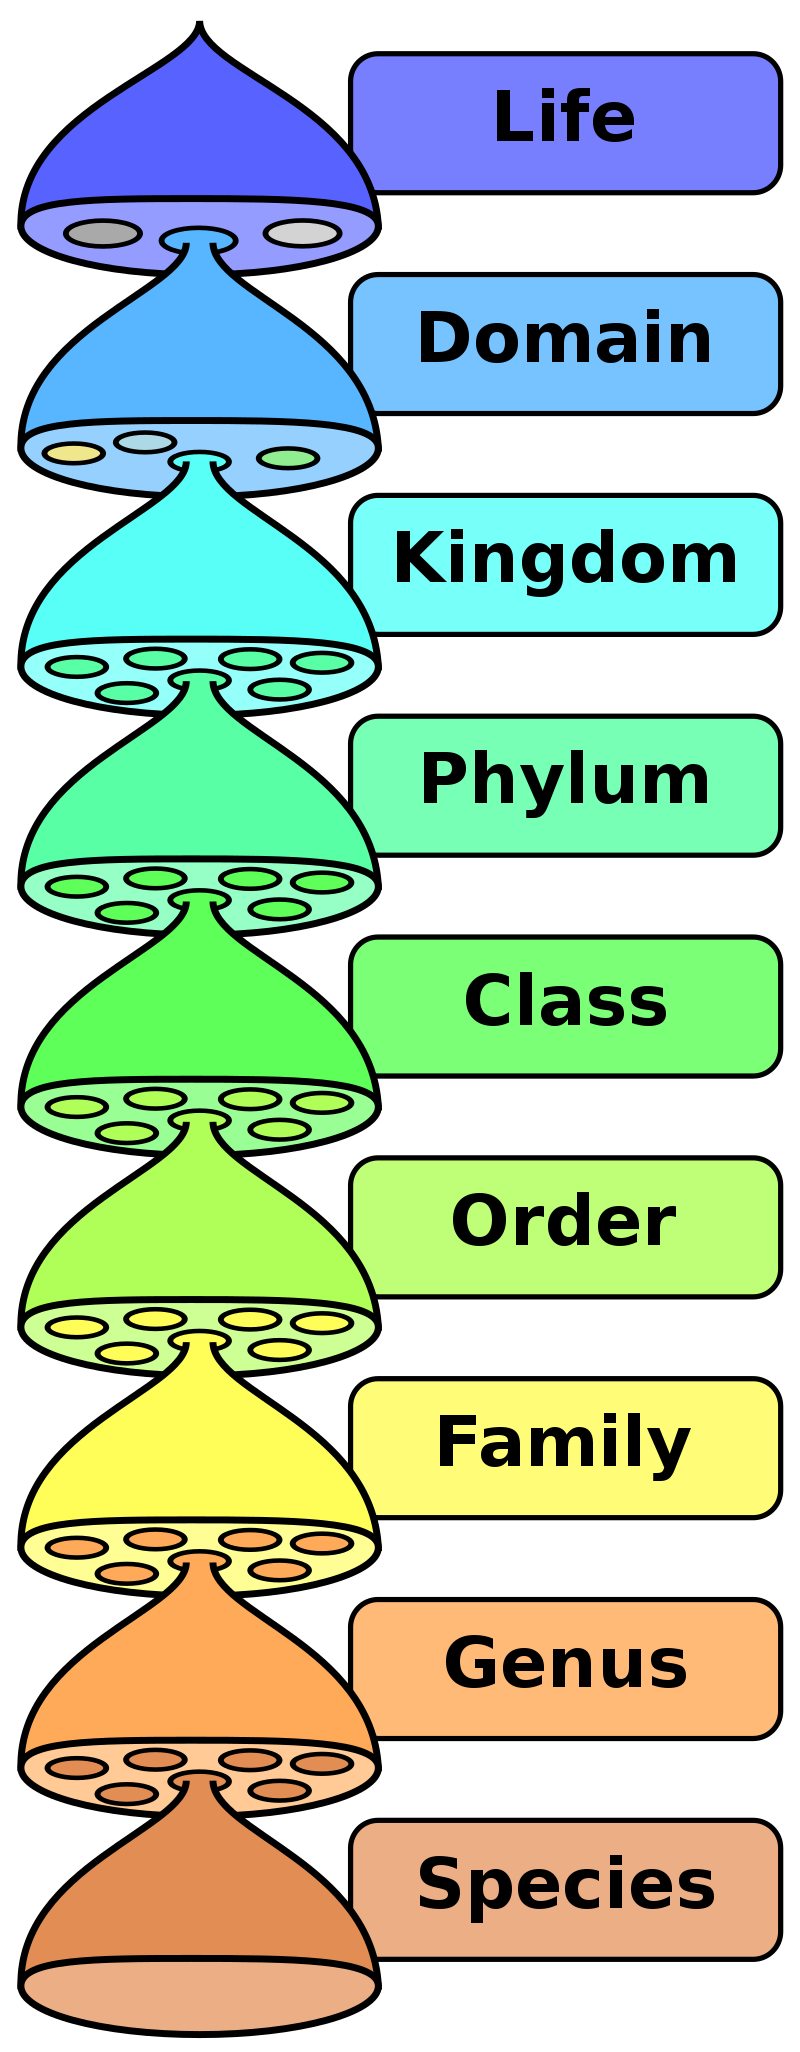
\includegraphics[width=1.0cm]{figures/class1.png}
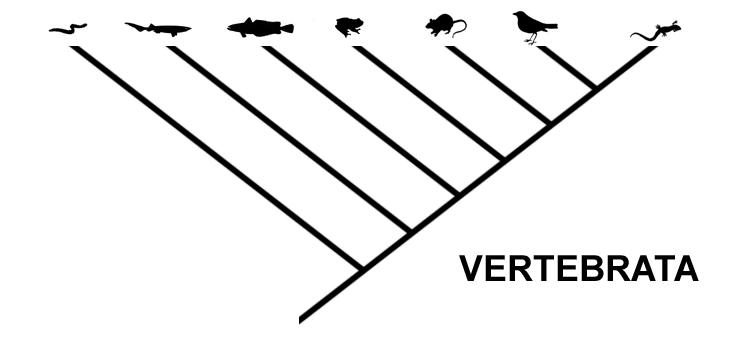
\includegraphics[width=3cm]{figures/class2.jpg}
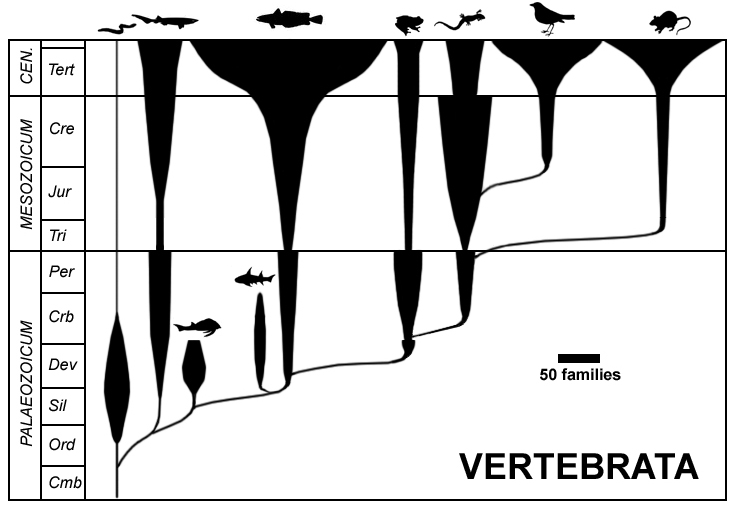
\includegraphics[width=3cm]{figures/class3.jpg}
\caption{(Far Left) A portrait of Carl Linnaeus (1707 - 1778).  (Left) Diagram of modern classification scheme. (Right) A cladogram detailing common ancestry. (Far right) Spindle diagram used for evolutionary taxonomy.}
\end{figure}
\small
\begin{itemize}
\item Expedition to Lapland
\item Invented modern latin binomial classification scheme
\item \textit{The Origin of Species} by Charles Darwin was published in 1859.
\end{itemize}
\end{frame}

\begin{frame}{Indigenous Medicine and Science}
\small
\textbf{Huitzilin}: hummingbird.  A discussion of Linnaean classification.  This species is completely restricted to the New World, so it would have been totally unknown to colonials.
\begin{itemize}
\item quetzal huitzilin (a quetzal is not a hummingbird)
\item xi huitzilin ... turquiose hummingbird
\item chalchi huitzilin ... light greed hummingbird
\item yiauhtic huitzilin ... purple hummingbird
\item tlapal huitzilin ... mixed black hummingbird
\item aiopal huitzilin ... light purple hummingbird
\item tle huitzilin ... hot coal colored hummingbird
\item quapa huitzilin ... tawny yellow hummingbird
\end{itemize}
The Nahua believed that hummingbirds are symbols of the warrior and immortality (torpor).
\end{frame}


\section{The Four Humors}

\begin{frame}{The Four Humors}
\textbf{\alert{The Four Humors}}: A medieval theory of medicine based on four classes of fluids within the body.  Each had an associated color.  Each color had a temperature classification, and a moisture classification.
\begin{figure}
\centering
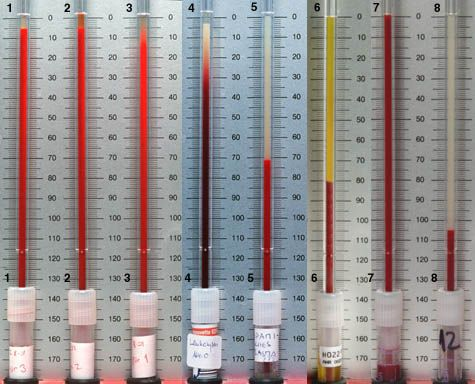
\includegraphics[width=5cm]{figures/blood1.jpg}
\caption{\label{fig:blood1} Blood sedimentation suggests that blood is built from sub-components that have different colors.}
\end{figure}
\end{frame}

\begin{frame}{The Four Humors}
\textbf{\alert{The Four Humors}}: A medieval theory of medicine based on four classes of fluids within the body.  Each had an associated color.  Each color had a temperature classification, and a moisture classification.
\begin{figure}
\centering
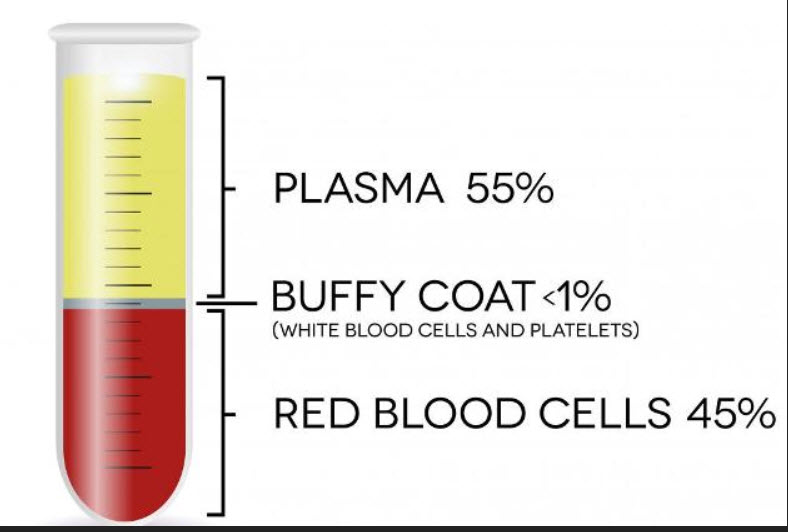
\includegraphics[width=5cm]{figures/blood2.jpg}
\caption{\label{fig:blood2} We now know that blood is in fact comprised of different substances: red blood cells, platelets, plasma, water, etc.}
\end{figure}
\end{frame}

\begin{frame}{The Four Humors}
\textbf{\alert{The Four Humors}}: Medieval scholars took it a step further and tried to associate the humors with the fundamental elements, based on the idea that we consume them to live.  Each food item or herb had a classification of hot/cold, and moist/dry.
\begin{figure}
\centering
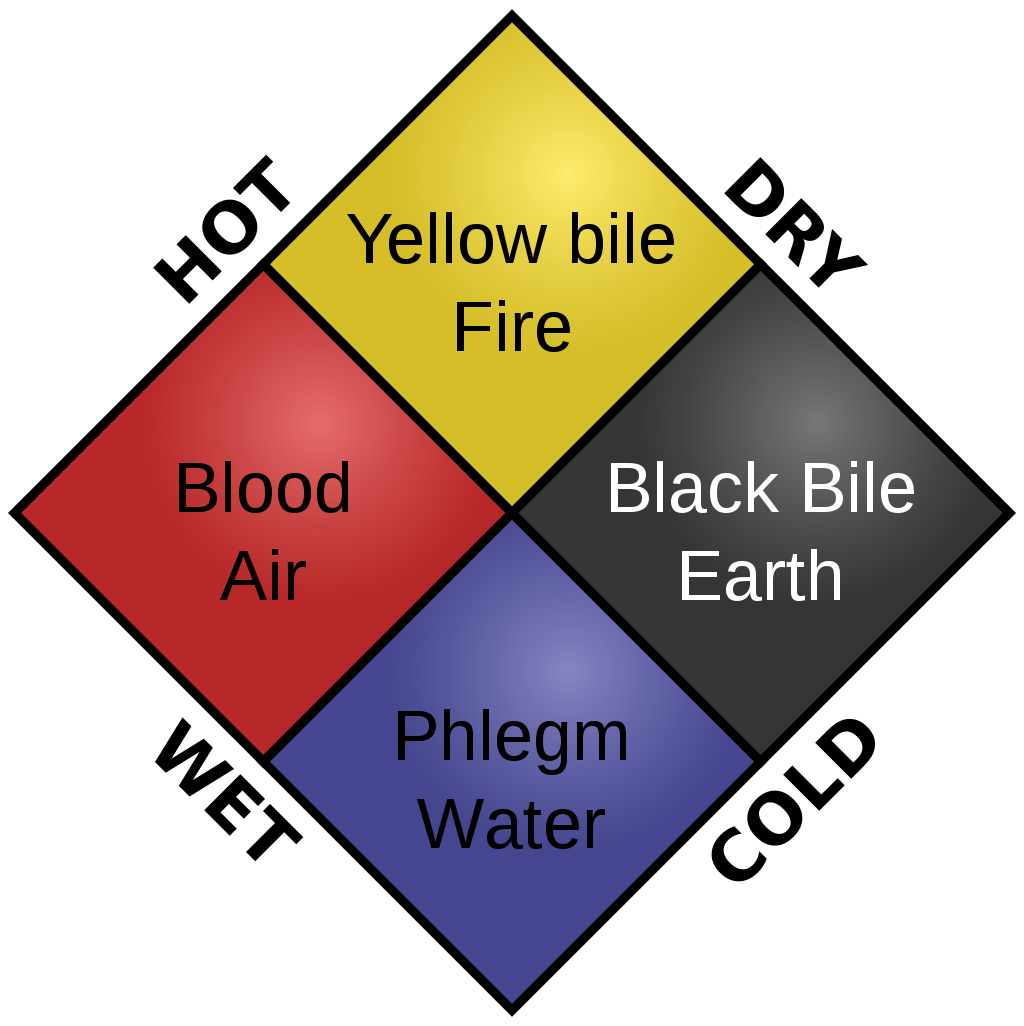
\includegraphics[width=3cm]{figures/humors.png}
\caption{\label{fig:humors} The four elements of the world were associated with the four humors, and further classified as hot/cold, and moist/dry.}
\end{figure}
\end{frame}

\begin{frame}{The Four Humors}
\small
It was even common up to the 18th century to explain personality traits using humor theory.  For a funny example of the intersection of popular culture and the four humors, see \\ \vspace{0.25cm} \url{https://youtu.be/dtsmluPK7Ug}
\begin{figure}
\centering

\includegraphics[width=3cm]{figures/turtles.jpg}
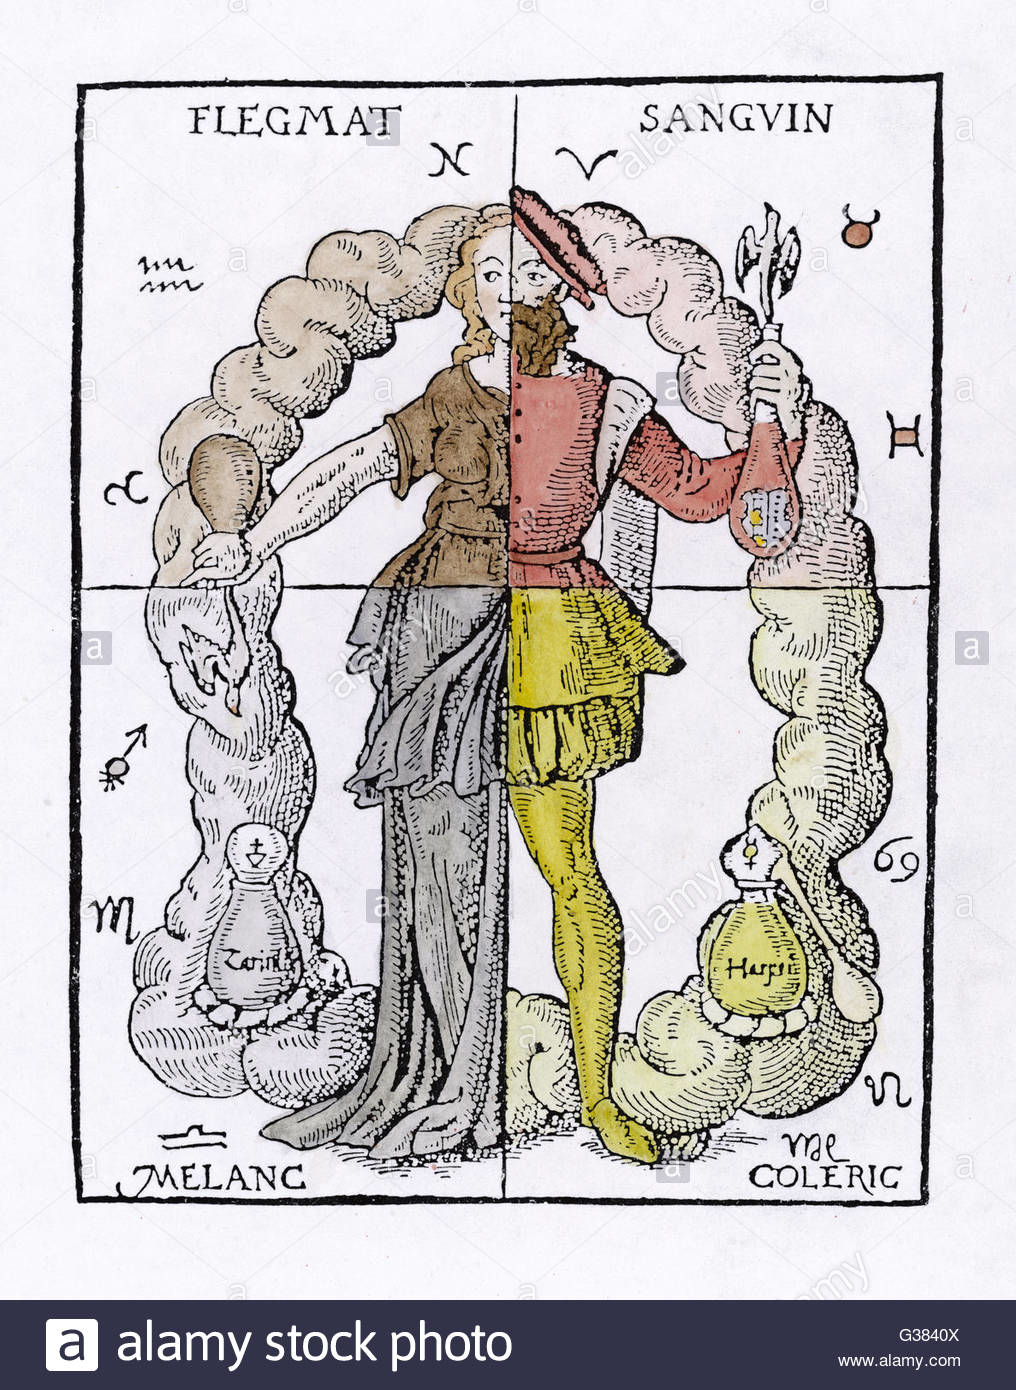
\includegraphics[width=3cm]{figures/traits.png}
\caption{\label{fig:humors2} The four humors were also associated with personality traits.}
\end{figure}
\end{frame}

\begin{frame}{The Four Humors}
\small
\alert{\textbf{Indigenous treatments were classified into this system}, but it did not always fit}.  According to an analysis by Juan de C\'{a}rdenas (1563-1609)\footnote{\url{https://es.wikipedia.org/wiki/Juan_de_C\%C3\%A1rdenas}}, the classification of cacao was complex:
\begin{enumerate}
\item Cacao is classified as \textit{cold and dry}, from the following observations:
\begin{itemize}
\item Bowel constriction and closing urinary tract
\item Stopping menstruation
\item Digestive problems
\end{itemize}
\item Chocolate is classified as \textit{warm and damp}, from the following observations:
\begin{itemize}
\item Chocolate is roasted and ground cacao mixed with \textit{atole}
\item Helps digestion, appetite
\item Helps bowel movement and urination
\end{itemize}
\end{enumerate}
\end{frame}

\begin{frame}{The Four Humors}
\small
\alert{\textbf{Indigenous treatments were classified into this system}, but it did not always fit}.  According to an analysis by Juan de C\'{a}rdenas (1563-1609)\footnote{\url{https://es.wikipedia.org/wiki/Juan_de_C\%C3\%A1rdenas}}, the classification of cacao was complex:
\begin{enumerate}
\item Chocolate is classified as \textit{warm and damp}
\item Theorizes that cacao has \textit{a third component, very hot and wet}:
\begin{itemize}
\item When cacao is plain, the cold restrictive effects
\item Roasted and mixed with atole, mild effects, and it tastes like chocolate
\item A third part, which causes sweating, triggers menstruation and digestive effects ... I wonder if this is the \textit{caffiene}
\end{itemize}
\item The explanation for the chemistry, though, is convoluted: the oily warm part removes some dryness from the hot part ...
\end{enumerate}
\end{frame}

\begin{frame}{The Four Humors}
\small
There are 12 mg of caffeine per 5.4 grams of cacao. \\ \vspace{0.5cm}

\includegraphics[width=8cm]{figures/menses.png}
\begin{itemize}
\item Caffeine consumption related to length of menstrual period
\item Caffeine consumption related to length of cycle
\item (This study is from 1999 and is part interview data, part chemical analysis)
\end{itemize}
What is interesting is how humor theory is being fit with the indigenous science.
\end{frame}

\begin{frame}{The Four Humors}
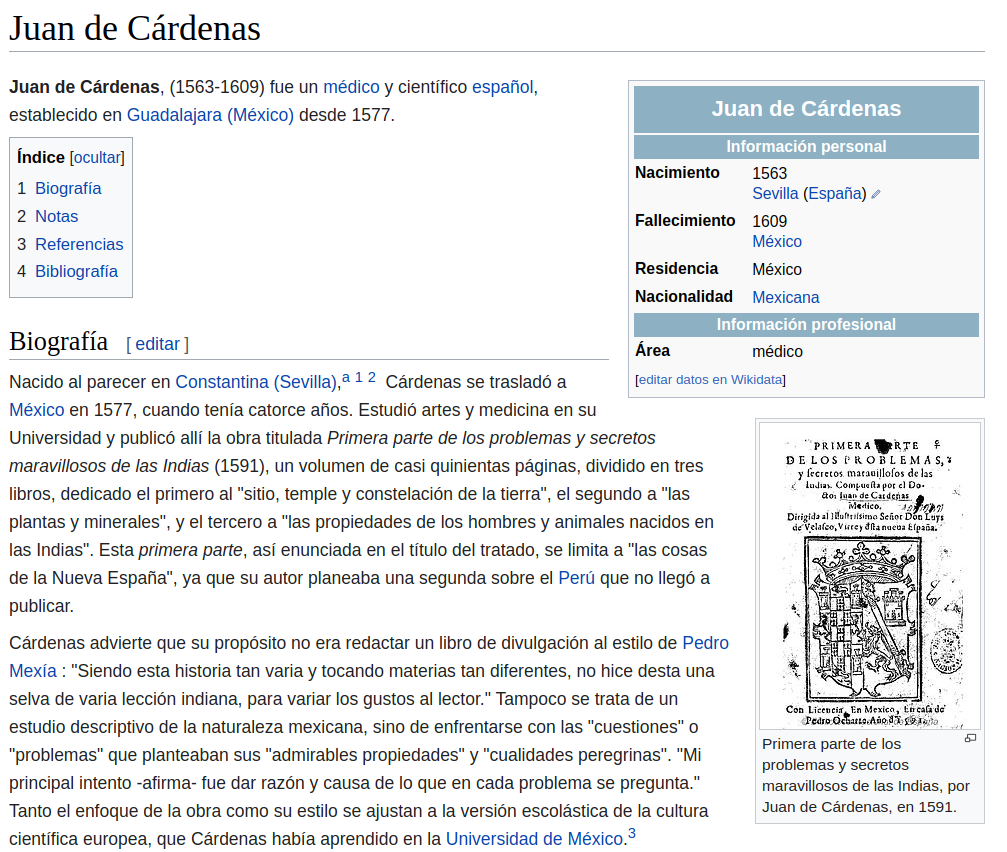
\includegraphics[width=9cm]{figures/cardenas.png}
\end{frame}

\section{Other Indigenous Treatments}

%\begin{frame}{Other Indigenous Treatmnts}
%\begin{figure}
%\centering
%\includegraphics[width=7cm]{figures/syphilis.jpg}
%\caption{Treponema pallidum - syphilis}
%\end{figure}
%\end{frame}

\begin{frame}{Other Indigenous Treatments}
Treatments for syphilis:
\begin{enumerate}
\item Bark of chinaberry tree
\item Root of sarsaparilla
\end{enumerate}
Spawned an entire industry of export to Europe.  Note in the text:
\begin{enumerate}
\item The Spaniards received this medicinal knowledge from the Native Americans
\item The cures worked, to some extent
\item Economic demand increased throughout the world
\item Europeans believed the cure originates near the source (not necessarily)
\end{enumerate}
\end{frame}

\begin{frame}{Indigenous Medicine and Science}
\small
\begin{enumerate}
\item \textbf{Xilo, xiloxochitl}: balsam, balsam tree.  A general term for residue extracted from tree matter that has medicinal properties.  The word balsam comes from The Balm of Gilead, in the Hebrew Bible (Genesis) for a region currently in Jordan.  Why did the Spanish colonials refer to \textit{xilo} as balsam?
\item \textbf{tzipipatli}: an herb native to Nueva Espa\~{n}a used to treat diarrhea.  Compare to how the Europeans treated diarrhea.  What is to be learned from the different treatments?
\end{enumerate}
\end{frame}

\begin{frame}{Other Indigenous Treatments}
Usages of balsam oil:
\begin{enumerate}
\item The Spaniards received this medicinal knowledge from the Native Americans
\item Prevention of scabies (antiseptic)
\item Sore muscles
\item Anti-inflammatory
\item Digestion
\item Prevention of rheumatism
\end{enumerate}
Cinchona bark:
\begin{enumerate}
\item Used in the production of quinine
\item Anti-malarial
\end{enumerate}
\textbf{Project ideas:} the writings of Nicol\'{a}s Monardes
\end{frame}

\section{Comparisons of Treatments}

\section{Conclusion}

\end{document}